%Appendix_power_distribution

This section aims for offering a set of numerical functions to calculating the power distribution along beam propagation in a photonic waveguide. The simplest idea is to compute the power in waveguide and base by integrating power flow density (or Poynting vector $\vec{S}$) at their cross-sections respectively. Meanwhile CST MWS has constructed a cuboid like Fig.\quad\ref{Afig:app_power_distribution01}, which contains all involved objects such as waveguide and TLF, as a total calculation space which is discretized through Finite Integral method (FIT) and all variables(see \cite{script_FeldSim} or section Finite Integration Method) from FIT are also available from CST MWS. In following it will be introduced how to calculate the power distribution of a Fiber-to-Chip model (see chapter modelling). 
\begin{figure}[ht]
\centering
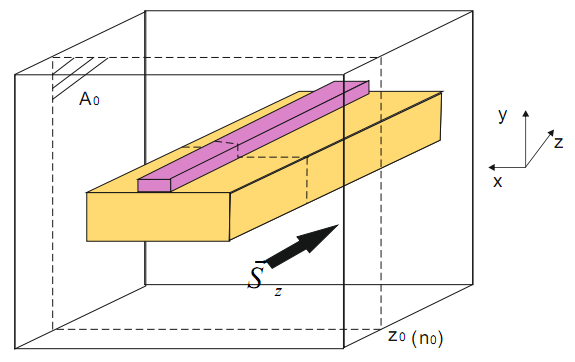
\includegraphics[width=0.7 \textwidth]{bilder/app_power_distribution01}
\caption{Calculation Cuboid in CST}
\label{Afig:app_power_distribution01}
\end{figure}
The first step is to choose a working plane. Suppose a working plane through point z$_{0}$ at z axis in the total calculation space Fig.\quad\ref{Afig:app_power_distribution01} is given, the point index n$_{0}$ can be determined by its coordinate z$_{0}$. The plane Fig. \quad\ref{Afig:app_power_distribution02}  is divided into small elemental pieces in FIT. The base cross-section is given by four points coordinates (x$_{1}$, y$_{1}$),(x$_{2}$, y$_{2}$),(x$_{3}$, y$_{3}$) and (x$_{4}$, y$_{4}$). Their points indexes (n$_{1}$, n$_{2}$, n$_{3}$, n$_{4}$) can also be derived.    
\begin{figure}[ht]
\centering
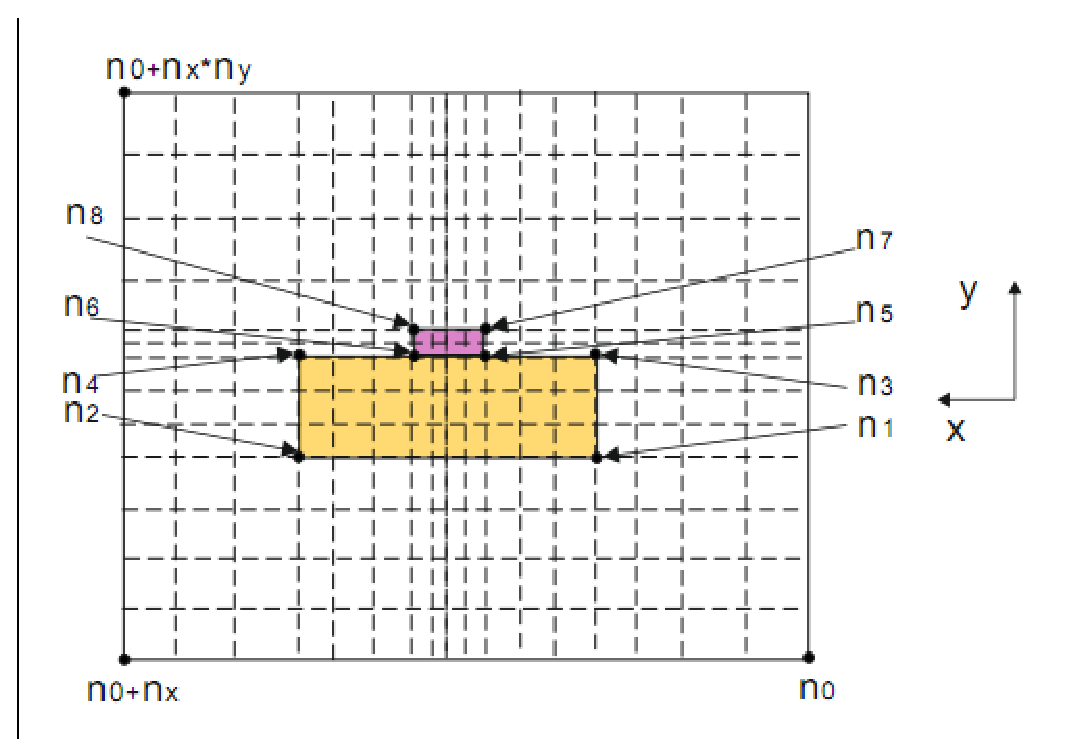
\includegraphics[width=0.7 \textwidth]{bilder/app_power_distribution02}
\caption{Cross-section at z$_{0}$}
\label{Afig:app_power_distribution02}
\end{figure}
In the next step it is necessary to prepare variables such as elemental 
As is in \cite{script_FeldSim} the complete elemental plane matrix D$_{A}$ is given by (\ref{Aeq:da_matrix}): 
\begin{equation}
D_{A}=Diag\left\{Ax(1),\cdots,Ax(Np),Ay(1),\cdots,Ay(Np), Az(1),\cdots,Az(Np)\right\}
\label{Aeq:da_matrix}
\end{equation}

In the working cross-section only z-components of elemental plane matrix D$_{A}$ are needed:
\begin{equation}
D_{Az}=D_{A}(2*Np+1:3*Np, 2*Np+1:3*Np)
\label{Aeq:daz_matrix}
\end{equation}
Construct a auxiliary matrix $A_{base}$, which composed of only $1$ and $0$ like Fig\quad\ref{Afig:app_Auxiliary_matrix}, to indicate all points indexes which are included in base cross-section. 

\begin{equation}
A_{base}=Diag\left\{0,\cdots 0,P_{1},0,\cdots 0, P_{2}, 0,\cdots, P_{m}, 0\cdots\right\}
\label{Aeq:A_matrix}
\end{equation}

\begin{figure}[!ht]
\centering
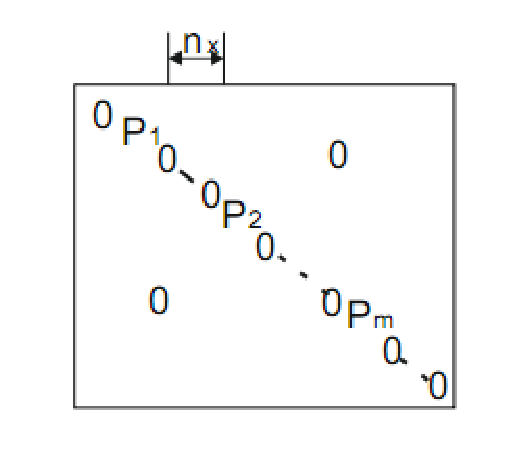
\includegraphics[width=0.5\textwidth]{bilder/app_Auxiliary_matrix}
\caption{structure of the auxiliary matrix $A$}
\label{Afig:app_Auxiliary_matrix}
\end{figure}
Where P$_{x}$ are submateix:
\begin{equation}
P_{x}=Diag\left\{1,\cdot,1\right\}_{(n_{2}-n_{1})*(n_{2}-n_{1})}
\end{equation}
And m is given by:
\begin{equation}
m=(n_{3}-n_{1})/n_{x}=(n_{4}-n_{2})/n_{x}
\end{equation}
Then 
\begin{equation}
D_{Abase}=A_{guide}*D_{A}
\end{equation}
Pick z-components of the Poynting vector $S$:
\begin{equation}
S_{z}=S(2*Np+1:3*Np)
\end{equation}
At last the power in base at the plane (for z=z$_{0}$) can be counted up by:
\begin{equation}
P_{base}(z)=sum(D_{Abase}*S_{z})
\end{equation}

By analogous procedures power in guide cross-section$P_{guide}$ and in total cross-section $P_{total}$ are derived. For observing the power distribution the results are processed by normalization:
\begin{align}
\eta_{guide}&=\frac{P_{guide}}{P_{total}}\\
\eta_{base}&=\frac{P_{base}}{P_{total}}\\
\eta_{air}&=1-\eta_{guide}-\eta_{base}
\end{align}

